\label{chapter:problem-description}
\chapter{Problem Description}

The goal of this thesis project is to help Tribler mature from an experimental research prototype into production-level code with potentially reliable usage by millions of users.\\\\
After careful analysis it was decided that within the context of a nine month project the strongest contribution to the future of Tribler would be a step forward in technical debt. At this point we believe the project does not need a particular focus on feature improvements, novel additional features, or boosting performance. After over ten years of software development by 44 unique contributors the amount of accumulated technical debt is worrying.\\\\
Tribler suffers from all kinds of technical debt, including code smells, coding style violations, code complexity and feature pollution in the graphical user interface. There is even a dedicated file, called \emph{hacks.py} that facilitates some workarounds caused by incompatible software.\\\\
This thesis is focussed on a round of invasive maintenance and cleaning of the code and all other infrastructure such as installers and testing environment. Our work aims to ensure that it is possible to conduct another decade of experimental distributed systems research with the Tribler code base. The alternative is continued usage and expansion of the code, which are likely to lead to a forced clean slate approach.\\\\
The structural problem is the lack of maintenance capacity. Each contributor to the Tribler research in the form of a bachelor, master, or PhD student needs to be primarily focussed on their thesis work. A thesis requires concrete experimental results, contribution to theory, or both. We believe the lack of student enthusiasm for fixing bugs and writing documentation is the root cause of current state of the code base.\\\\
In this remaining of this chapter, various problems within the Tribler project will be highlighted.

\section{A large code base}
Tribler has a very large, complex code base. This makes Tribler an unattractive open-source project for external developers since the process to get familiar with the code base takes a long time. Figure \ref{fig:openhub-commits} illustrates the number of commits over the past 10 years. The evolution of number of source code lines is shown in Figure \ref{fig:openhub-loc}. The magnitude of the project is also presented by Figure \ref{fig:openhub-commit-stats}. From these figures, it is clear that Tribler has continued to grow to a project with an unmaintainable amount of code. According to the basic COCOMO model, the established costs of the project is \$2,371,403 with an estimated effort of 43 person-years.\\\\
This continue growth can be explained by the fact that Tribler is a research-oriented prototype. Students often contribute to Tribler by implementing a specific feature of the system, such as anonymous downloads, credit mining mechanisms or an adult filter to filter out explicit content. After completions of these features, the student leaves the project and the knowledge about the specific part of Tribler he or she contributed to, is lost. Afterwards, that part of Tribler is not maintained anymore, due to lack of knowledge and manpower constraints.\\\\
Continuous expansion of a system inevitably leads to feature pollution. During the past 10 years, no single effort has been made to do a proper clean up of the current code. The code base contains a huge amount of technical debt. If this trend continues, Tribler will evolve into an tremendously complex system where the choice to use a clean-slate approach is favoured over continued usage of the current code base.

\begin{figure}[!h]
	\centering
	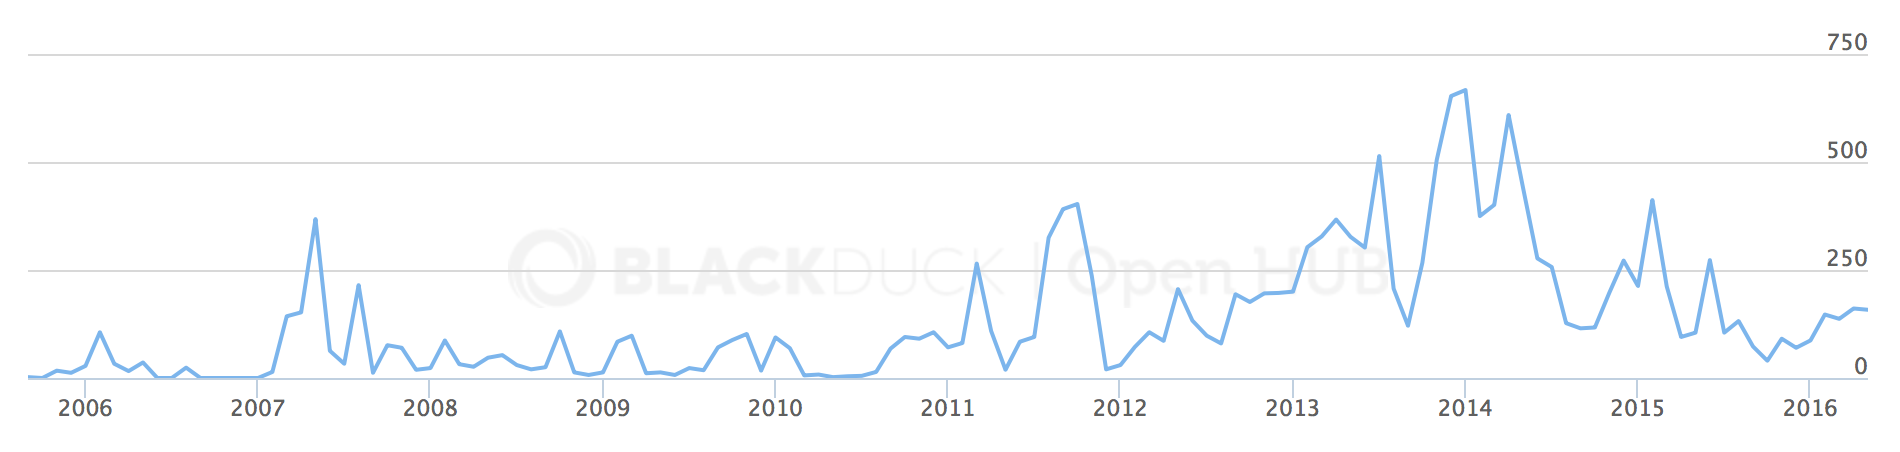
\includegraphics[width=\columnwidth]{images/openhub_commits}
	\caption{An history of commits on the Tribler project, as reported by OpenHub.}
	\label{fig:openhub-commits}
\end{figure}

\begin{figure}[!h]
	\centering
	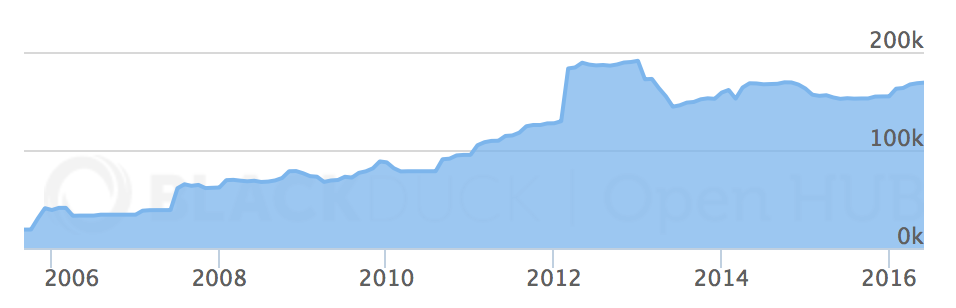
\includegraphics[width=\columnwidth]{images/openhub_loc}
	\caption{The evolution of lines of code in the Tribler project, as reported by OpenHub.}
	\label{fig:openhub-loc}
\end{figure}

\begin{figure}[!h]
	\centering
	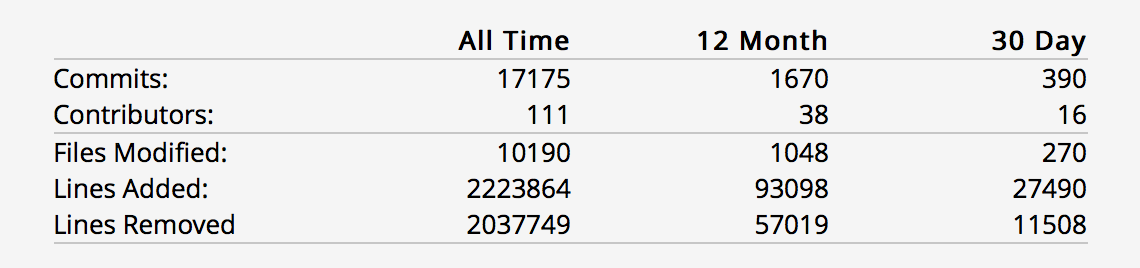
\includegraphics[width=0.6\columnwidth]{images/openhub_commits_table}
	\caption{Statistics about modifications to the code base, as reported by OpenHub.}
	\label{fig:openhub-commit-stats}
\end{figure}

\section{Lack of Maintenance}
Many features of Tribler are completely unmaintained, due to lack of knowledge or resource constraints. There are even some experimental features that are not working anymore and could be removed.\\\\
The lack of maintenance is clearly visible in the synchronization system of Tribler, called \emph{Dispersy}. Dispersy is a platform to simplify the design of distributed communities and is mostly designed and written by
N. Zeilemaker and B. Schoon\cite{zeilemaker2013dispersy}. After these two developers left the project, knowledge of the Dispersy system disappeared and the system transited to an unmaintained state.\\\\
Most researchers working with Tribler have a specific feature to deliver. This means that defects in unmaintained parts of Tribler are not prioritized, causing long outstanding issues on GitHub that are not resolved and delayed for many major or minor release. Of the 300 total issues on GitHub, 100 issues are older than one year.
 
\section{Architectural Impurity}
During the lifetime of Tribler, the architecture has been subject to various minor and major modifications. Starting as a fork from ABC, a Bittorrent client based on Bittornado, Tribler has evolved to a platform that allows users to discover, share and download content. The evolution of the architecture of Tribler will be explained in-depth in Chapter \ref{chapter:architecture}.\\\\
On the highest code-base level, two main components in Tribler can be identified: the module with code providing the graphical user interface and the code that contains the core of Tribler. These modules have a mutual dependency on each other which is considered bad design since the Tribler core should never be dependent on the user interface. Splitting this dependency is a high priority issue.\\\\
Overall, the code base feels like a bunch of glued together research works whereby every developer maintained his own code style and practices. No clear design patterns can be identified throughout the code and there is a staggering amount of legacy code that is either unused or can be removed.\\\\
After more analysis of the core module, we managed to identify some other issues. Code that facilitates a video player is present in the core package while this is clearly related to the user interface. We have two files with configuration parameters that can easily be merged to reduce complexity and increase maintainability.\\\\
The code related to the graphical user interface is highly coupled and of poor quality. While the current decade of software engineering provides a plethora of visual designers that requires barely any hand-written code, our whole graphical user interface is built with code that's unmaintained and hard to read. Many features and visual elements in the graphical user interface are unnecessary and unintuitive, contributing to the technical debt. Finally, the user interface has been written with the \emph{wxPython} framework which is not maintained anymore since late 2014. The library builds upon native APIs, i.e. Cocoa on OS X and Win32 on Windows. While the library claims to be cross-platform with a native look and feel, various features in Tribler are limited to a subset of the supported platforms.
\todo{add import graph with cycles}

\section{Unstable and incomplete testing framework}
Proper testing is the responsibility of every developer. Over the past 10 years, this responsibility has been completely neglected by the majority of the contributors. Tribler has a structural lack of proper designed unit tests. Currently, around 100 tests are available. Many of these tests are taking over half a minute to complete and are bootstrapping an extensive Tribler session. Only a small fraction of the test suite has the characteristics of unit tests. Having tests that are doing a broad range of operations, inevitably leads to undesired side-effect and failing tests. No single attempt has been made to mock components of the system to simplify tests and focus on the part of the system that has to be verified.\\\\
There is one more factor that contributes to the instability of the current test suite. A significant part of the test suite is depending on external network resources, ranging from trackers and seeders for a specific torrent to other peers in the decentralized network. This fragile architecture gives rise to failing tests due to unavailable nodes, unexpected responses from external peers and other unpredicted circumstances.\\\\
In general, well designed tests exclude any dependency on external resource that is outside the control of the developer. This can be achieved by mocking method calls to return dummy data. Additionally, one can make sure that the external resource is available in the local testing environment. For instance, when a test is dependent on a specific torrent seeder, a local libtorrent session can be started that seeds this torrent.\\\\
While Tribler is packaged and distributed for multiple platforms, unit tests in our continuous integration environment are only executed on a machine running a Linux operating system. Limiting test execution to one platform, lowers the overall code coverage and covers platform-specific bugs. Attention should be given to make our test execution multi-platform.\\\\
% http://shhetri.github.io/unit-testing-to-tackle-technical-debt/
Right unit testing can also be used as tool to tackle technical debt. Unit testing makes the developer directly responsible for producing working code, even before it reaches the review phase. It helps to discover bugs and errors in a more early stage of development and gives more insight in the amount of technical debt that one will accumulate by making a short-term decision. % todo beter uitleggen?

%\section{Quality Assurance}
%The ongoing lack of any quality assurance measure has led to several concerns. In this Section, some of the problems regarding quality assurance will be addressed.
%
%\subsection{Test Suite}
%Tribler has a structural lack of proper designed unit tests. Currently, there are 99 tests and 48.970 lines of code in the Tribler module (excluding code in the Dispersy framework). Many of these tests are taking over half a minute to complete and are bootstrapping an extensive Tribler session. Only a small fraction of the test suite has the characteristics of unit tests. Having tests that are doing a broad range of operations, inevitably leads to undesired side-effect and failing tests. No single attempt has been made to mock components of the system to simplify tests and focus on the part of the system that has to be verified.\\\\
%To illustrate this problematic situation in more detail, the tunnel community is taken as example. The tunnel community allows users of Tribler to anonymously download content and is one of the most anticipated features of the software. The current test suite contains no single unit test that is focussed on this part of the code. Instead, there are several unstable integration-like tests that are starting up a graphical user interface and perform an anonymous download. While one might argue that having such a test might be sufficient for regression testing purposes, this test does not fully cover the source code and any code related to error handling is completely uncovered.\\\\
%There is one more factor that contributes to the instability of the current test suite. A significant part of the test suite is depending on external network resources, ranging from trackers and seeders for a specific torrent to other peers in the decentralized Dispersy network. This fragile architecture gives rise to failing tests due to unavailable nodes, unexpected responses from external peers and other unpredicted circumstances.\\\\
%In general, well designed tests exclude any dependency on external resource that is outside the control of the developer. This can be achieved by mocking method calls to return dummy data. Additionally, one can make sure that the external resource is available in the local testing environment. For instance, when a test is dependent on a specific torrent seeder, a local libtorrent session can be started that seeds this torrent.
%
%\subsection{Testing Environment}
%Tribler uses a Jenkins environment to automate the testing of new Pull Requests (PRs). These tests are only executed on a Linux server. Tribler itself, however, is also packaged and distributed for Windows and OS X. According to the GitHub download statistics, the Windows and OS X distributions account for 91\% of the downloads\footnote{https://api.github.com/repos/tribler/tribler/releases/latest}. Not running any test on this platform is a missed opportunity to identify platform-specific errors. Moreover, any conditional in the source code that is only executed on a specific platform, remains completely uncovered and untested.
%
%\subsection{Documentation}
%The responsibility to maintain a proper and up-to-date documentation base for current and new developers has been completely neglected during the lifespan of the Tribler project. Except for some general information about the project, there is a minimal amount of information available about the system. Since the process of familiarization with the source code is very hard, Tribler has become an unattractive open-source project to contribute to.
%
%\subsection{Outdated Dependencies}
%The Tribler code base has many dependencies on other libraries. At the time of writing, Tribler depends on at least 20 other python libraries. Apart from that, we need libraries for testing and packaging the code. Keeping these libraries up to date, is a necessary and important process.\\\\
%Outdated libraries might lead to compatibility issues and workarounds. For packaging Tribler on Windows, we are using \emph{py2exe}, a library that is not maintained since 2008. Usage of \emph{py2exe} might be dropped in favor of more maintained and mature libraries, for instance, \emph{PyInstaller}.
%
%
%\section{Code quality}
%In the previous Section, the lack of quality assurance and the consequences of this has been elaborated. In this Section, the focus will shift to the code itself. Identified issues in the current structure of the source code will be discussed.
%
%\subsection{Graphical User Interface}
%The current Graphical User Interface (GUI) of Tribler is written with the wxPython library. The GUI accounts for just over 20.000 source lines of code (SLOC), making up 33\% of the Tribler code base which is significant.\\\\
%The code base of the GUI is has been subject to various refactoring cycles. This leads to a very complex and hard to understand package of code. Technical debt is clearly visible in this part of the code base. Moreover, the interface is plagued with many useless and hidden features that are contributing to the complexity of the code. A clean slate approach with a more mature and user-friendly libraries seems to be the solution that could benefit Tribler the most.\\\\
%The current decade of software engineering provides many alternative tools and libraries that allows to build a visually appealing, platform-independent interface with a minimal amount of code. For instance, the popular and mature Qt framework allows developers to specify their layout in a visual designer.
%
%\subsection{High Coupling between modules}
%The user interface and core of Tribler are interleaved to such an extent that it is inconvenient for developers to test out specific features without making changes to the GUI. Providing a minimal Tribler service that only runs the core code and removing the dependencies between the core and user interface will boost the productivity of developers. An interface can be provided to provide necessary  interactions with the core. There are some more occurrences of dependencies between modules which should be removed. For instance, a full Tribler session object is passed to the constructor of the main database class while a path to the destination location of the database file suffices.\\\\
%By separating modules from each other, the ease of maintainability can be improved since developers do not need to worry about errors that are propagating to other module dependencies. Separation also leads to a code base that is easier to understand.
%
%\subsection{Inconsistent Code Style}
%After the contribution of 44 developers, numerous code styles across the code base can be identified. This leads to an inconsistent code base. There is absolutely no appliance to the PEP8 guidelines which is based on the fact that the current source code contains a sheer amount of 1644 violations.

%Refactoring overview 5-pages

%This chapter show a general overview of all the various large and small contributions made to boost the health of the code base. In total over 13000 lines of code have been altered. 33 pull requests accepted.
%GUI screenshots, before, after
%remove DB calls from GUI.
%Github screenshots with altered lines of code.
%progressive JSON API.

%Quality Assurance infrastructure 8-pages

%In the previous chapter a general overview is provided of the numerous changes to the code base. Now we focus on the specific changes for quality assurance in more detail. Key change is 
%splitting of the code base into two parts to make them easier to maintain.  
%-documentation, easier to contribute, improved learning curve, REST API.
%software performance regresssion-graphs
%evolution of code coverage

%Experimental results 10-pages GRAPHS

%We now focus on performance experiments of our new Tribler code base and demonstrate the key improvements.

%Startup time graph, 10 runs + 10 runs new
% + breakdown, checkpoints..
%remote search
%download speed
%memory usage+stress test, while doing lots of REST API calls.
%content discovery speed, Subscribe channels experiment: 1,5,10,15,25 joined channels and resource usage.

%...